%%%%%%%%%%%%%%%%%%%%%%%%%%%%%%%%%%%%%%%%%%%%%%
\section{Les build-systèmes}
%%%%%%%%%%%%%%%%%%%%%%%%%%%%%%%%%%%%%%%%%%%%%%

\begin{frame}{Les différents travails en Linux embarqué}
  \begin{itemize}
  \item {\bf BSP}: portage du bootloader et du noyau Linux + développement de drivers.
  \item {\bf Integration système}: assembler tous les composents userspace nécessaires pour le système, les configurer, mécanismes de mise à jour, etc
  \item {\bf Développement applicatif}: écrire des applications ou librairies spécifiques à l'entreprise
  \end{itemize}
\end{frame}

\begin{frame}{Complexité de l'intégration userspace}
  \begin{center}
    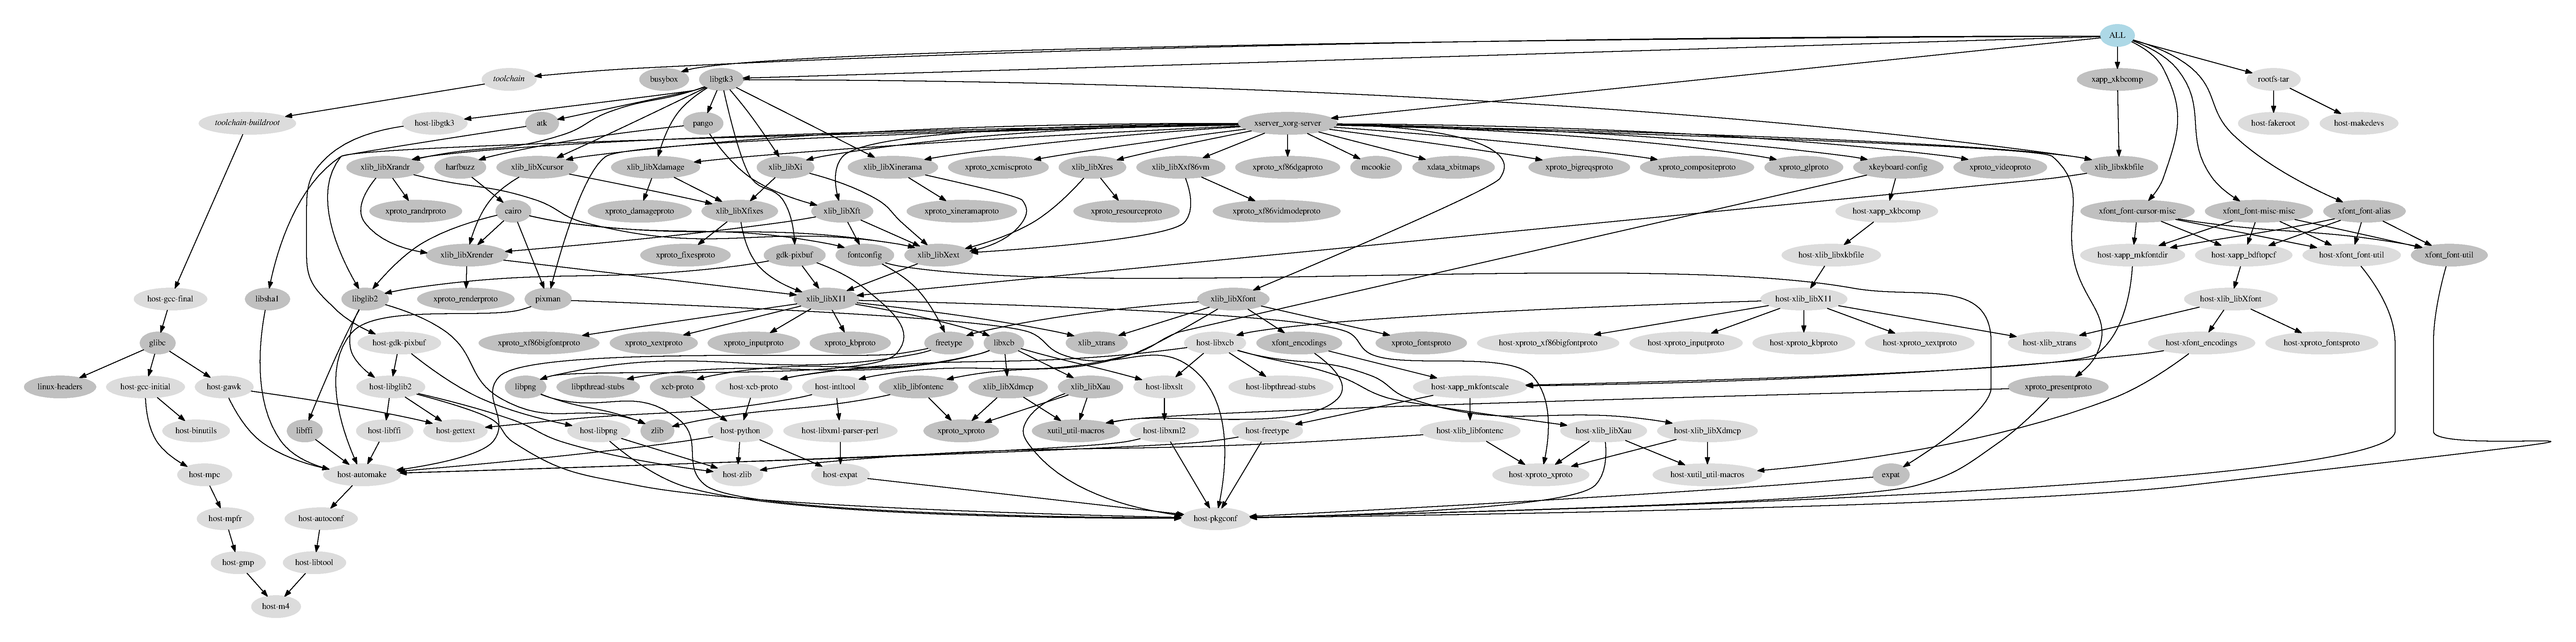
\includegraphics[width=\textwidth]{graphics/graph-depends.pdf}
  \end{center}
\end{frame}

\begin{frame}{Intégration système: plusieurs possibilités}
  \tiny
  \begin{tabularx}{14cm}{|X|X|X|}
    \hline
    & {\bf Pros} & {\bf Cons} \\
    \hline
    {\bf Compiler tout manuellement} &
    Complètement flexible \newline
    Gagne en expérience &
    Enfer des dépendances \newline
    Doit comprendre tout un tas de détails \newline
    Compatibilité des version \newline
    Manque de reproductibilité \\
    \hline
    {\bf Distributions binaires} \newline Debian, Ubuntu, Fedora, etc.
    &
    Facile à créer et étendre
    &
    Difficile à customiser \newline
    Difficile à optimizer (temps de boot, taille) \newline
    Difficile de compiler depuis les sources \newline
    Système gros \newline
    Compilation native \newline
    Pas de mécanisme bien définis pour générer une image \newline
    Pleins de dépendances obligatoires \newline
    Pas disponibles pour toutes les architectures \\
    \hline
    {\bf Systèmes de build} \newline Buildroot, Yocto, PTXdist, etc.
    &
    Quasiment complètement flexible \newline
    Compile depuis les sources : customisation et optimisation faciles \newline
    Complètement reproductible \newline
    Cross-compilation \newline
    Contains des paquets spécifique à l'embarqué \newline
    &
    Pas aussi facile qu'une distribution binaire \newline
    Temps de build \\
    \hline
  \end{tabularx}
\end{frame}

\begin{frame}{Build system: principe}
  \begin{center}
    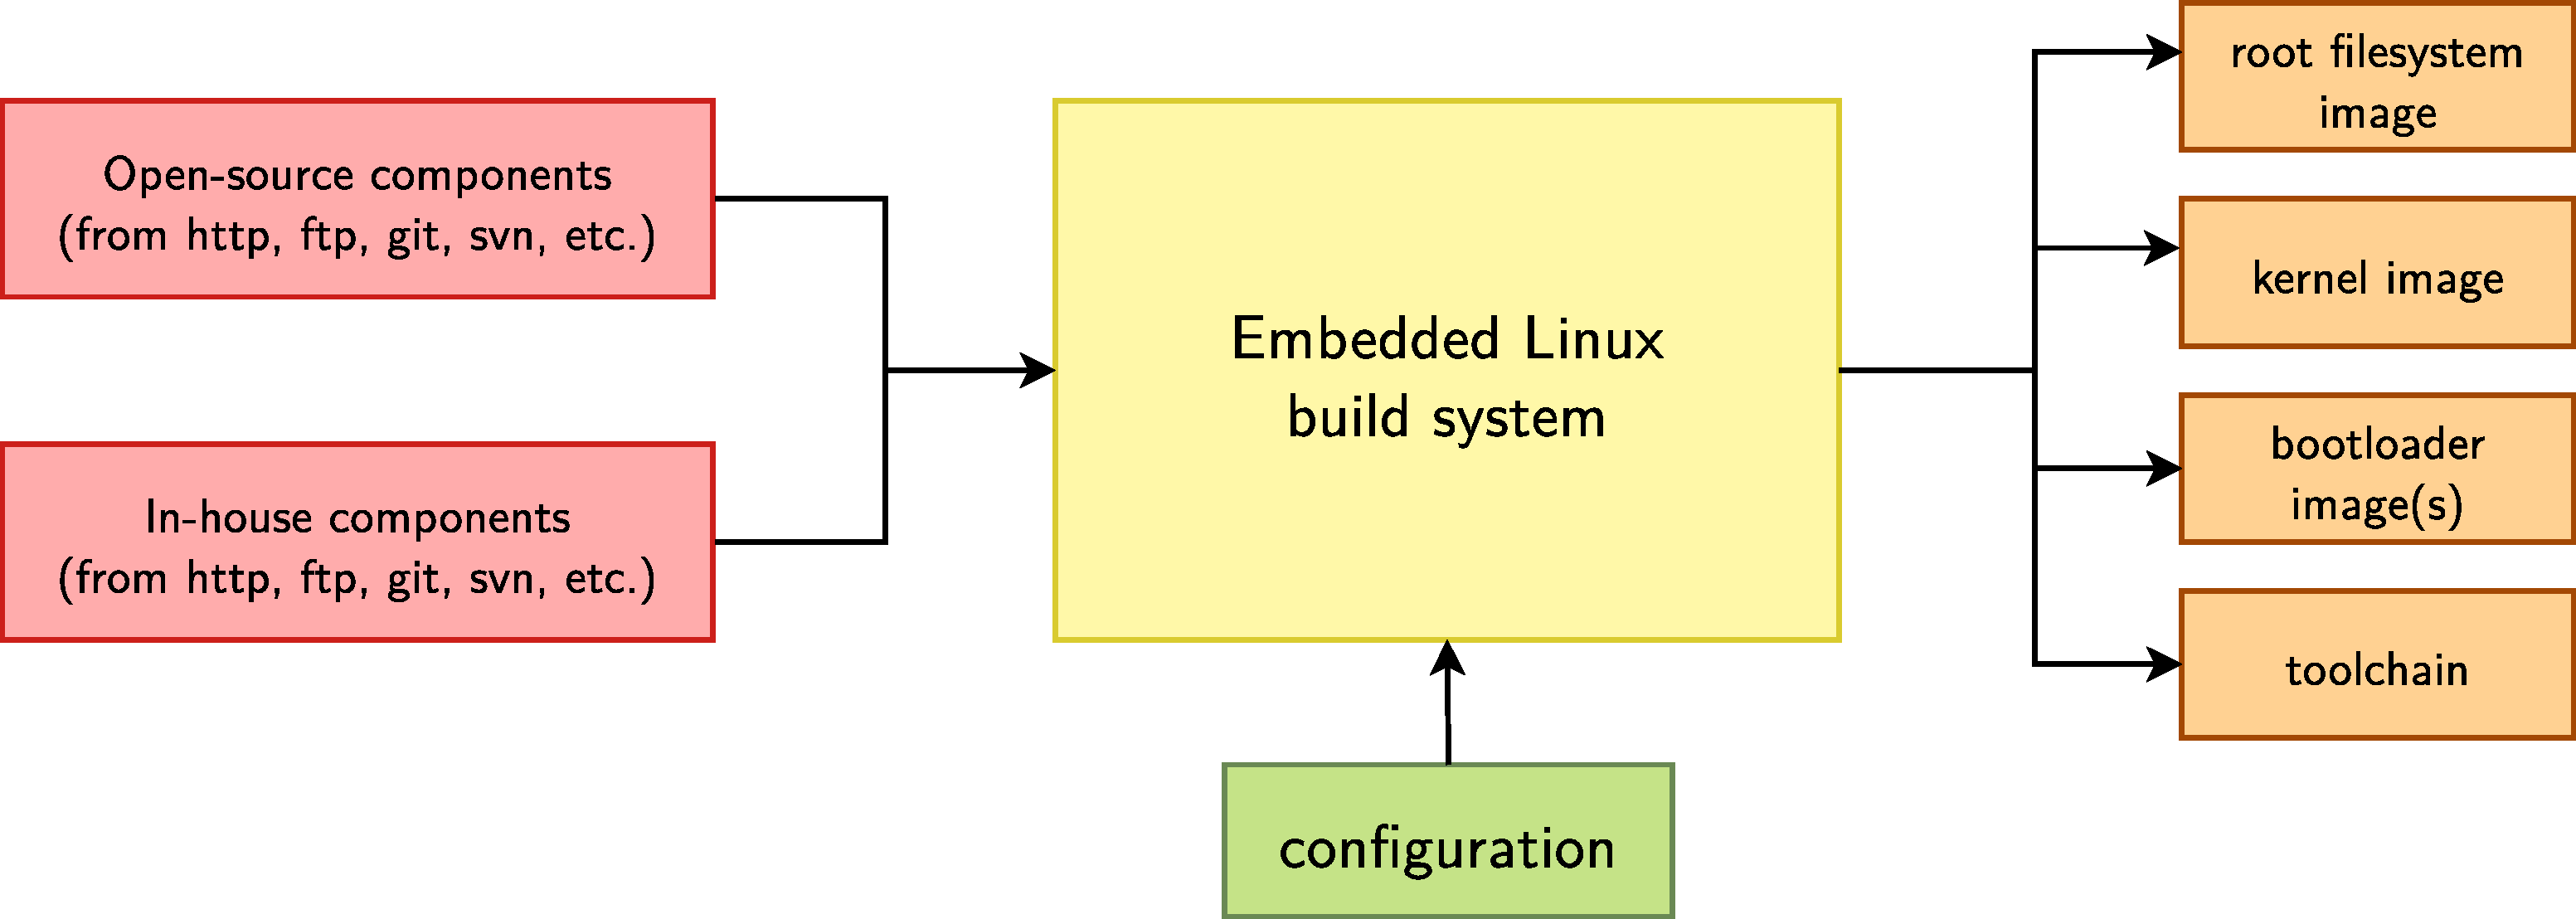
\includegraphics[width=0.9\textwidth]{graphics/buildsystem-principle.pdf}
  \end{center}
  \begin{itemize}
  \item Compilation depuis les sources $\rightarrow$ flexibilité
  \item Cross-compilation $\rightarrow$ rapidité à compiler si utilise des machines de build
  \item Recettes pour compiler des composants $\rightarrow$ facile
  \end{itemize}
\end{frame}

\begin{frame}{Les outils}
  \begin{itemize}
  \item Beaucoup de solutions possibles : Yocto/OpenEmbedded, PTXdist,
    Buildroot, OpenBricks, OpenWRT, etc.
  \item Mais 2 solutions émergent comme les plus populaires :
    \begin{itemize}
    \item {\bf Yocto/OpenEmbedded}\\Compile une distribution Linux complète avec des paquets binaires. Très puissant mais complexe et prend beaucoup de temps à apprendre
    \item {\bf Buildroot}\\Compile une image de rootfs, pas de paquets binaires. Beaucoup plus simple à utiliser, comprendre et modifier.
    \end{itemize}
  \end{itemize}
\end{frame}
